Модуль \texttt{packer} является частью сигнального процессора LASP и предназначен для вычисления необходимых энергетических сумм по узлам калориметра и последующей упаковки данных для отправки в целевую систему.\par
\begin{figure}[ht]
    \centering
    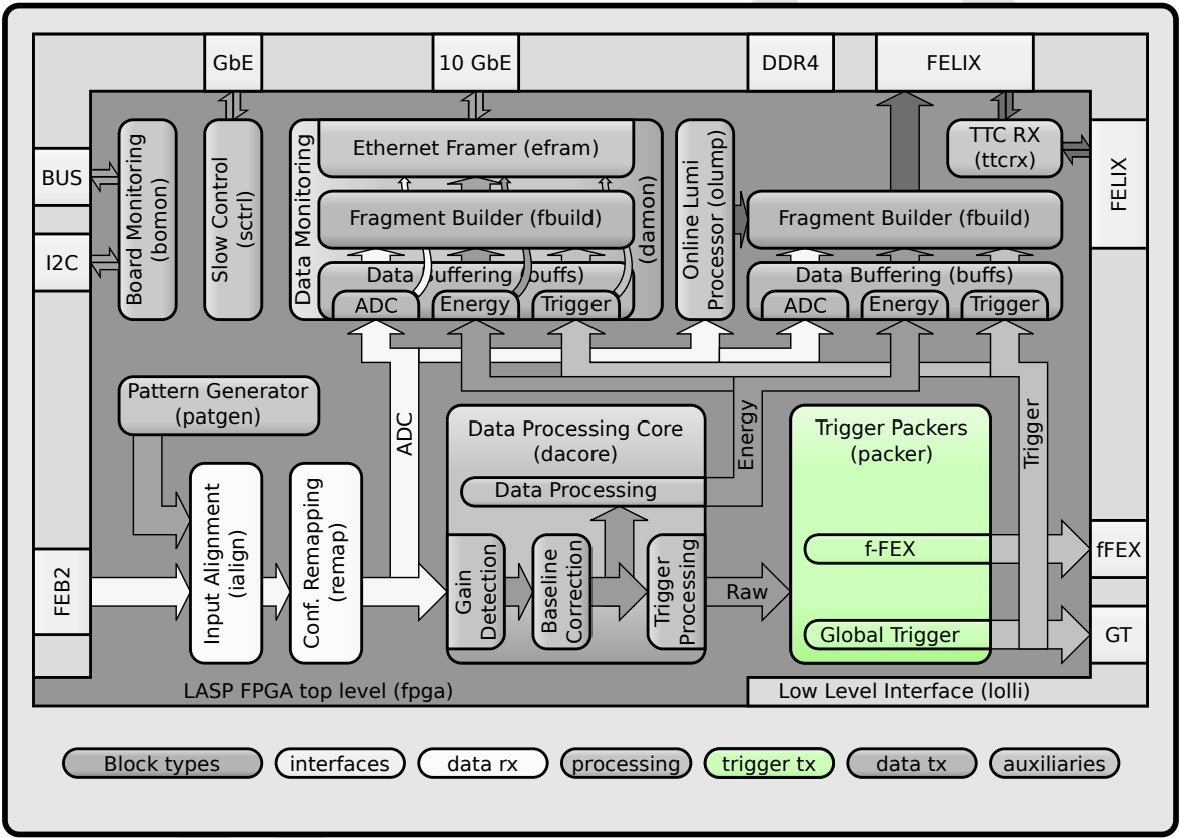
\includegraphics[width=0.8\linewidth]{packer_lasp.png}
    \caption{Схема расположения модуля packer в общей структуре сигнального процессора LASP}
    \label{fig:packer_lasp}
\end{figure}\par

Модуль \texttt{packer} обеспечивает данные для двух внешних подсистем: глобальный триггер и fFEX. Система fFEX \parencite{tdr_blue} является представителем набора модулей FEX, с помощью которых осуществляется поиск специфичных событий в ускорителе. Для этого ей не требуется полный объём данных, поступающих с детектора, а достаточно лишь определённой части, причём зачастую используются не конкретные значения, а суммы по целым участкам калориметра.\par
Для передачи данных во внешние подсистемы используется подход упаковки информации в кадры, которые уже непосредственно отправляются клиенту. Поскольку в системе сбора данных имеется жесткая система синхронизации -- приёмник и передатчик синхронизованы между собой и частотой БАК -- при передаче данных не требуется синхронизация в каждом пакете. Полоса пропускания полностью используется для передачи данных, упакованных в кадры, в каждом из которых содержатся данные от одного столкновния пучков. На рисунке \ref{fig:packer_ffex_frame} изображен один из предложенных вариантов формата кадра данных. Он содержит 46 десятибитных значений АЦП, идентификатор столкновения пучков, а также флаги превышения данными порога $2 \sigma$. Помимо представленного варианта также были предложения реализовать кадры с переменной структурой, которые наиболее эффективно использовали бы пропускную способность канала передачи данных для разных участков калориметра.\par
\begin{figure}[ht]
    \centering
    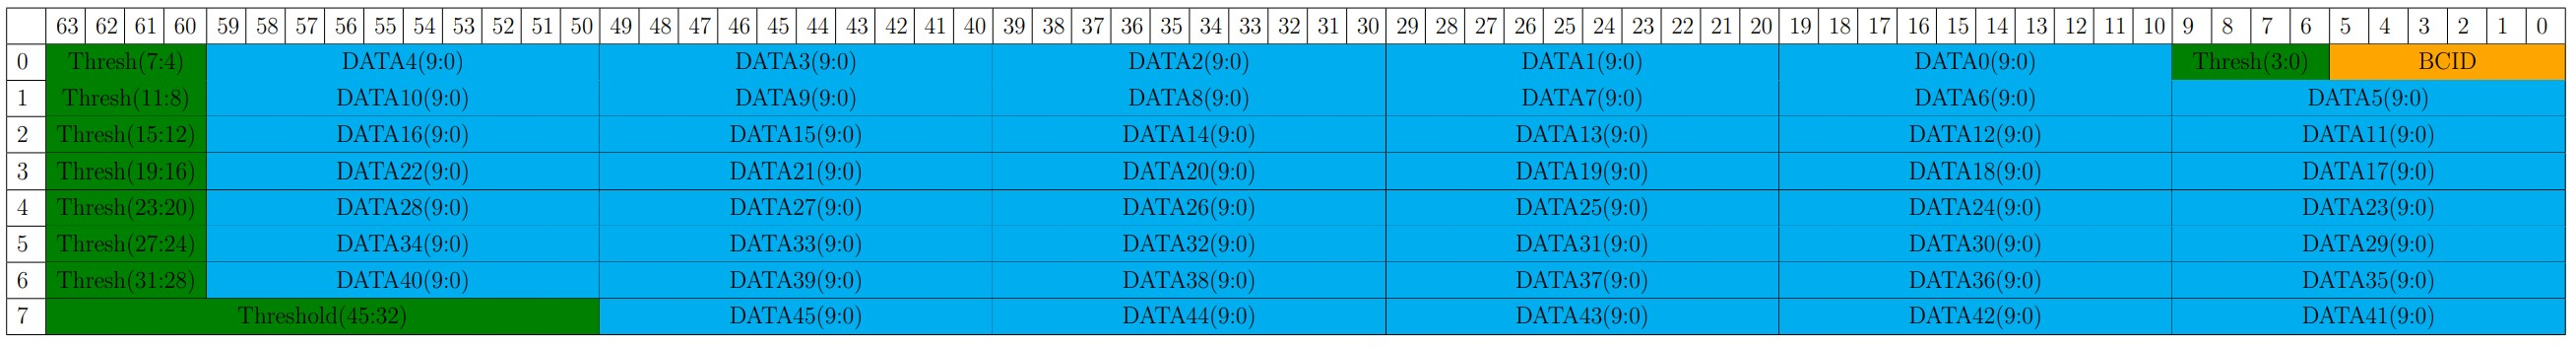
\includegraphics[width=\linewidth]{packer_ffex_frame.png}
    \caption{Вариант формата кадра данных для отправки в систему fFEX}
    \label{fig:packer_ffex_frame}
\end{figure}\par
В ходе работы был разработан прототип модуля \texttt{packer} на языке описания цифровой логики VHDL, и подготовлено тестовое симуляционное окружение для моделирования его поведения. Также этот модуль был интегрирован в общий дизайн сигнального процессора LASP в рамках подхода top-down \parencite{topdown}. Таким образом, весь дизайн целиком LASP сейчас может модулироваться и компилироваться. Целевая функциональность модуля упаковки триггерных данных будет реализована после согласования требований с разработчиками системы fFEX (ожидается в 2023).\par
